\documentclass{article}
\title{Electromagnetism Practical, Session 2\\Free Space Propagation of EM waves}
\author{Rijk van Wijk 4261569, Bart Kolling 4228219, Jasper Smit 4217527,\\ Ian Zhang 4243943}
\usepackage{graphicx}
\usepackage{float}
 \usepackage{epstopdf}
\usepackage[square,numbers]{natbib}
\usepackage{amsmath}
\usepackage{hyperref}
\usepackage{bookmark}
%\usepackage[margin=1cm]{fullwidth}
\usepackage{ gensymb }
\begin{document}

\maketitle

\newpage

\section{Assignment 1: Free space propagation}

	\subsection{Wavelength and propagation velocity in free space}
		The shift in position of the array translates to a shift in phase.
		The demodulator lets this phase shift slip for a fraction of a second, in which the 1kHz wave slips through the demodulator.
		This event can be seen on the scope or heard via the speaker.
		\newline
		The measured wavelength is $\lambda = 2*(0.017) = 3.4 cm$.
		The propagation speed will then be $v = f/\lambda = 3.11*10^8 m/s$

	\subsection{Measurement of the relation between the received signal and propagation distance}
		The power of the signal will decrease quadratically, like the surface of a sphere. 
		The voltage is proportional to the square root of the power, so the estimation is that the value of $x$ in equation \ref{11sigv} is unity.

		\begin{equation}
		\label{11sigv}
			V = \frac{const}{R^x}
		\end{equation}

		Looking at the results of table \ref{11vrx} and assuming $x = 1$, the constant will approximately be $0.25$.
		This brings us to a relation between the received signal voltage $V_{RX}$ and distance $R$ of $V_{RX} = \frac{1}{4\cdot R}$.


		\begin{table}[H]
			\centering
			\begin{tabular}{l|lllllll}
				Distance {[}m{]} & 0.10 & 0.20 & 0.30 & 0.40 & 0.50 & 0.60 & 0.70 \\ \hline
				Voltage {[}V{]}  & 2.16 & 1.38 & 0.96 & 0.74 & 0.60 & 0.48 & 0.38
			\end{tabular}
			\caption{The measured received voltages at various distances from the transmitter.}
			\label{11vrx}
		\end{table}

		\begin{figure}[H]
			\centering
			\label{11fig}
			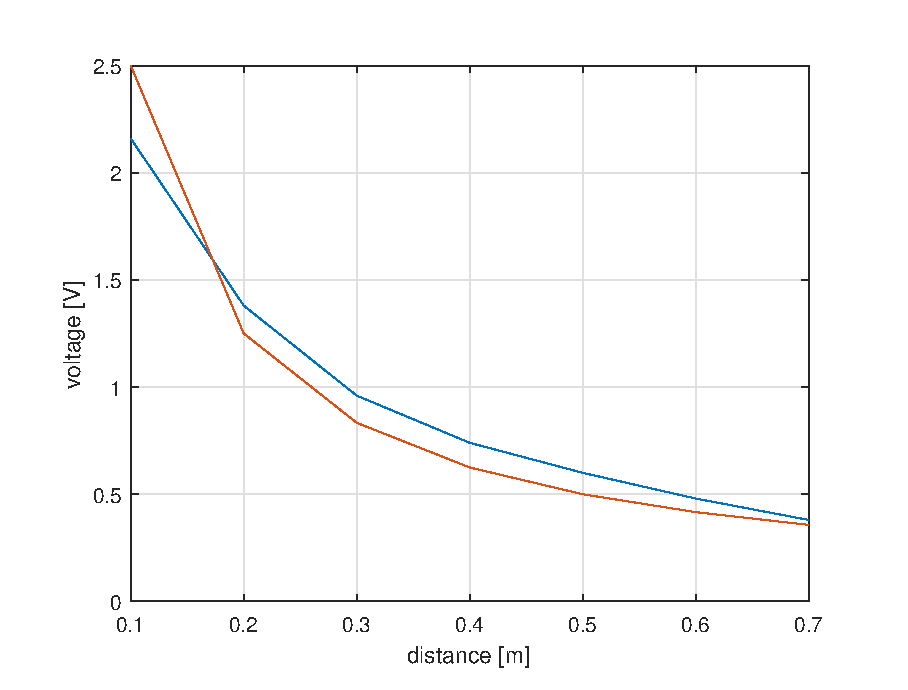
\includegraphics[width=0.7\textwidth]{Plotjes/ass11.eps}
			\caption{The measured voltages (blue) compared to the estimation (orange).}
		\end{figure}


	\subsection{Study of the transmission and absorption of EM waves on flat objects}
		This experiment covers placing different planar objects in the LOS and observing their reflective properties. 
		Table \ref{12vrx} displays the results.
		The metal plate absorbs the EM wave, so almost nothing is received.
		The absorbing material does the same, which is not surprising.
		The same goes for the vertical wires. 
		The horizontal wires, however, absorb even less than the dielectric.
		This is because the polarized signal is not affected by the horizontal wires and doesn't transition through another material for the most part.
		
		\begin{table}[H]
			\centering
			\begin{tabular}{l|llllll}
				% tabel met relative spanning
				%                     & No obstruction & Metal & Dielectric & Absorbing & Vertical wires & Horizontal wires \\ \hline
				% Voltage on receiver & 0.275          & 0     & 0.230      & 0.024     & 0              & 0.240            \\
				% Relative voltage    & 1              & 0     & 0.836      & 0.087     & 0              & 0.873           

				% tabel met relative power in dBW
				                       & Nothing        & Metal         & Dielectric & Absorbing & Vert. wires & Horiz. wires \\ \hline
				$V_{rx} {[}V{]} $        & 0.275          & 0             & 0.230      & 0.024     & 0              & 0.240            \\
				$P_{RX}/P_{0} {[}dB{]}$  & 0              & \textless -30 & -1.55      & -21.18    & \textless -30  & -1.18  
			\end{tabular}
			\caption{Signal voltages and relative signal power on the receiver.}
			\label{12vrx}
		\end{table}



	\subsection{The influence of polarization}
		The polarization isolation measured is $Q = -17.63dB$.
		\newline
		% het volgende is hierop gebaseerd http://alienryderflex.com/polarizer/
		The maximum received signal power is almost $50\%$ of the received signal power on a zero degree polarisation difference. 
		This result was achieved by placing the vertical wires at an angle of $45\degree$.
		The vertical wires act as an polarization filter by crushing the polarized signal to a $45\degree$ orientation. 
		Because of this, the magnitude drops to $cos(45\degree) = \sqrt{2}$ of the original signal.
		The receiver is also polarized, and oriented at $45\degree$ with respect to the wires, and so the same magnitude drop occurs at the receiver.
		This in total causes the transmitted signal to be weakened by a factor $\sqrt{2}*\sqrt{2} = 2$.






\section{Assignment 2: Measurements of the polarisation state of the EM Wave using
the polarization pattern method}


\subsection{Assignment 2.1}\label{ass21}
\begin{figure}[H]
\centering
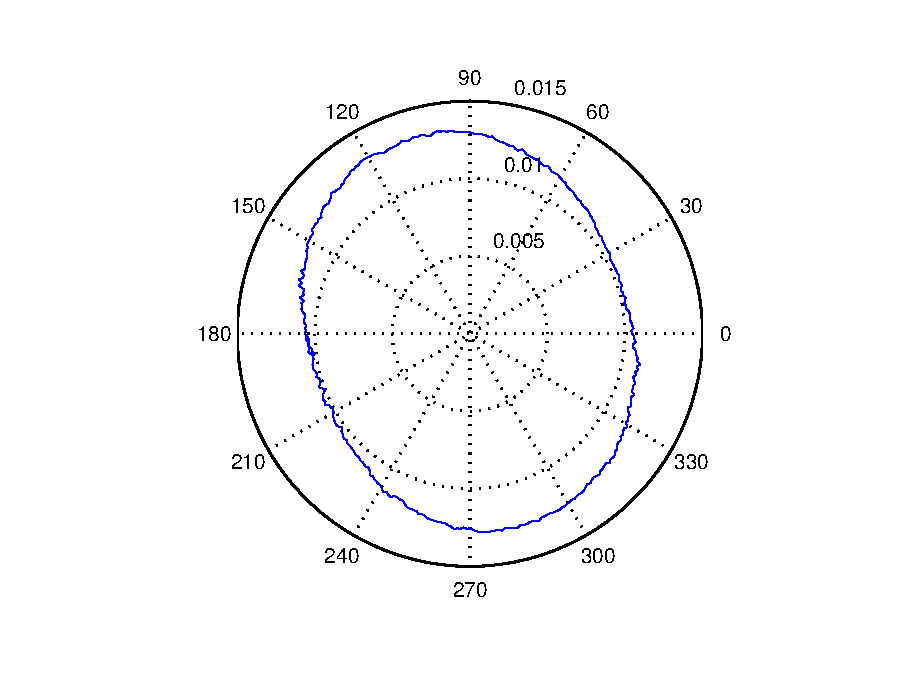
\includegraphics[width=0.7\textwidth]{Plotjes/ass21.eps}
\caption{Polarization pattern of a circular polarized wave with absorbing material to counter reflections }
\end{figure}

\begin{figure}[H]
\centering
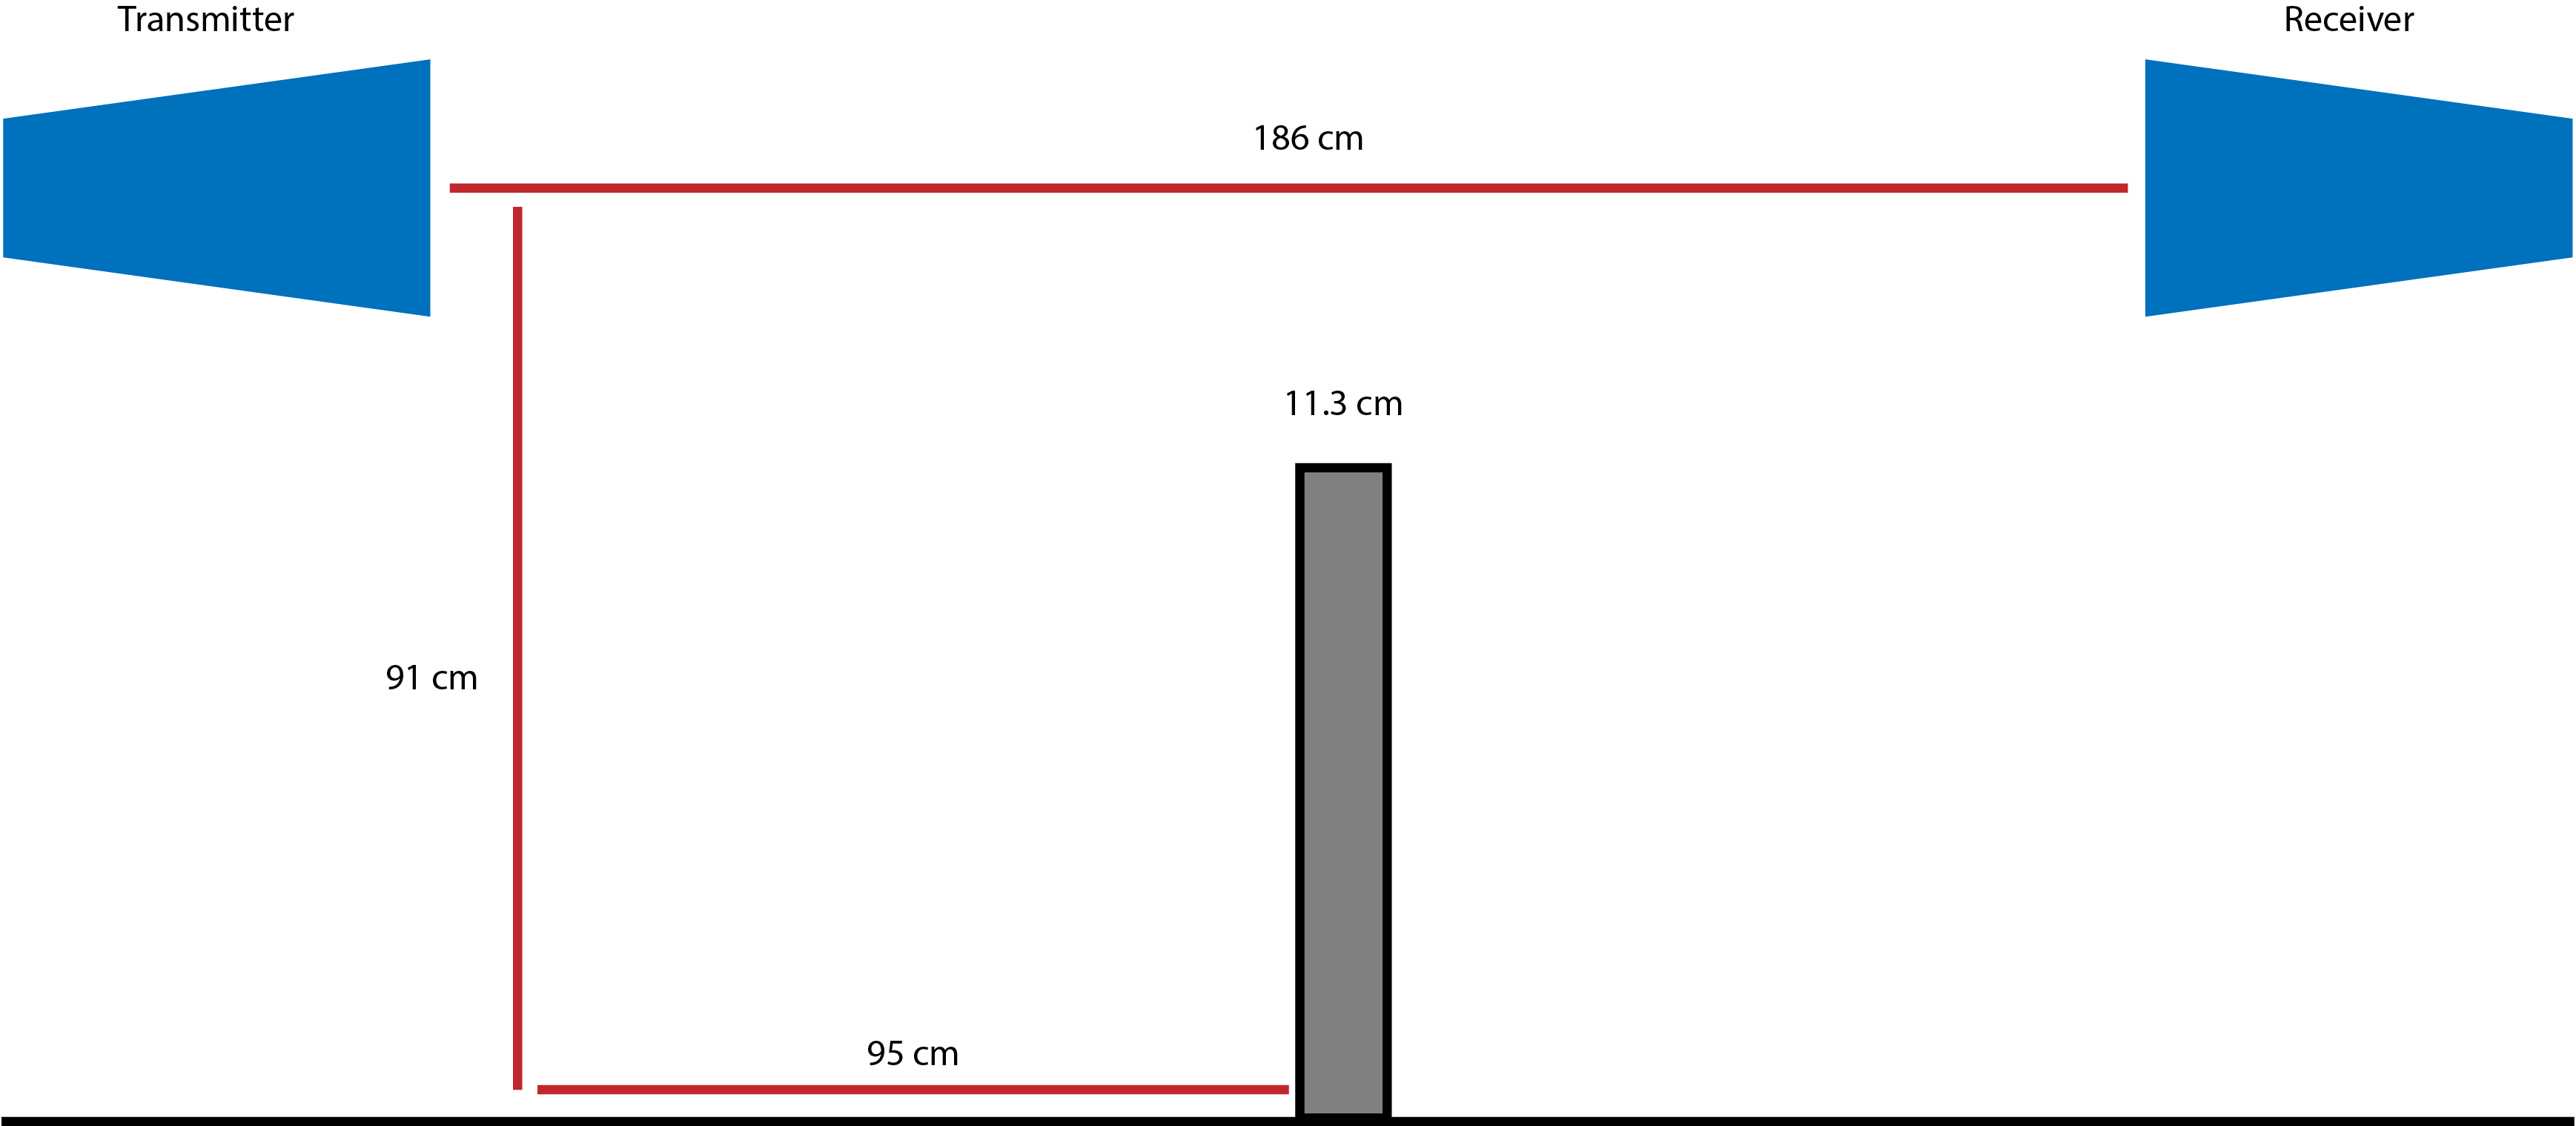
\includegraphics[width=\textwidth]{EM-1.png}
\caption{The setup of with the absorbing material with the measurements.}
\end{figure}

\begin{figure}[H]
\centering
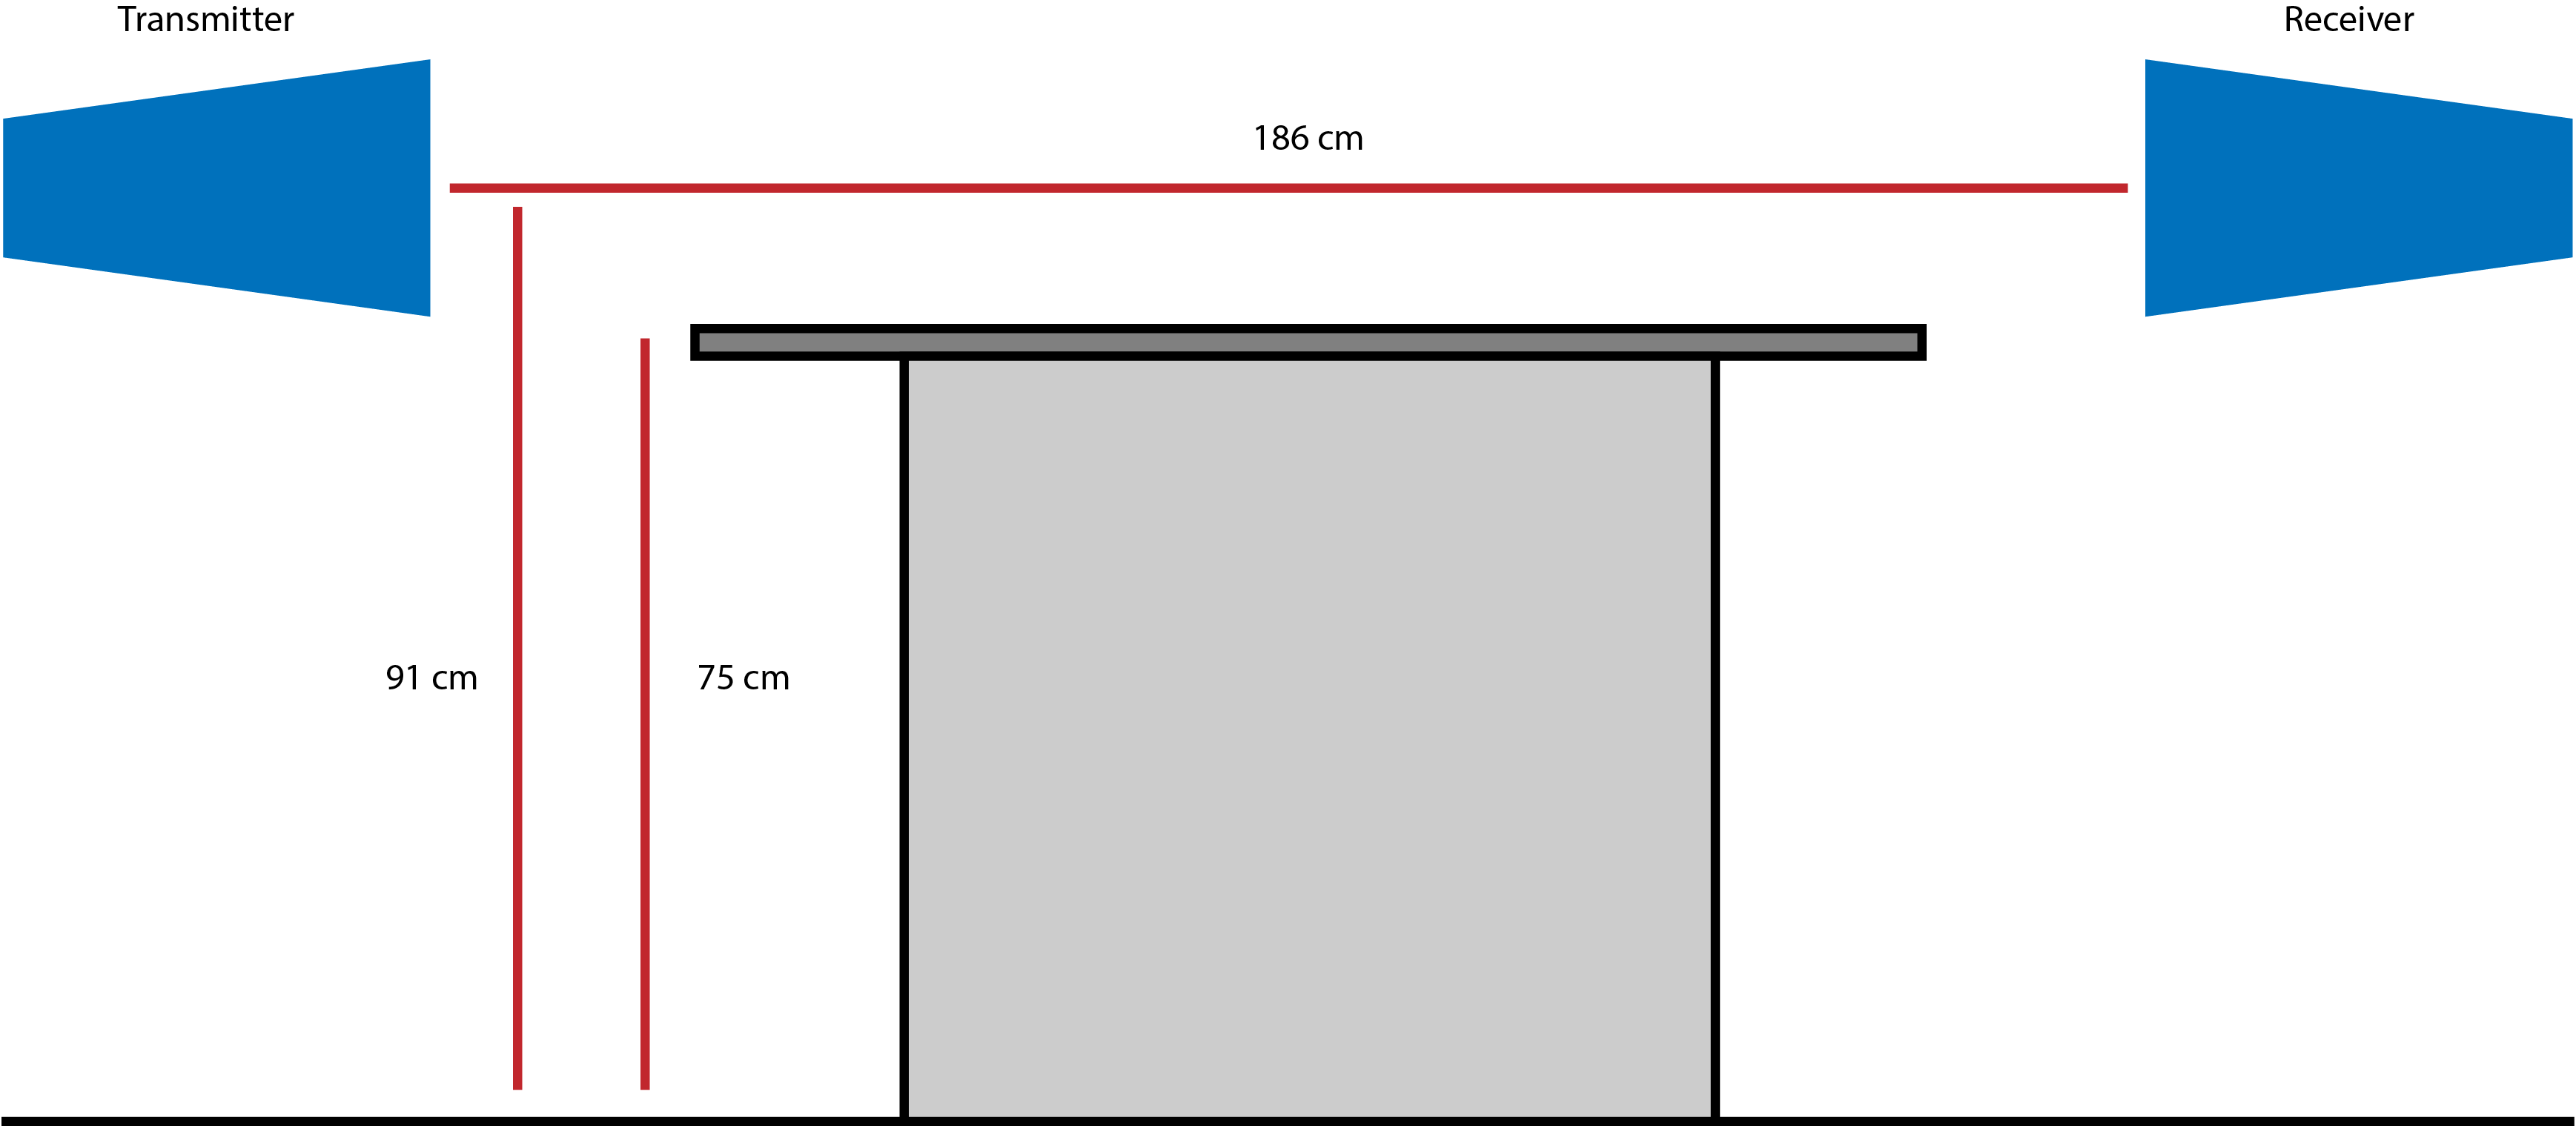
\includegraphics[width=\textwidth]{EM-2.png}
\caption{The setup of with the metal plate with the measurements.}
\end{figure}


\subsection{Assignment 2.2}\label{ass22}
\begin{figure}[H]
\centering
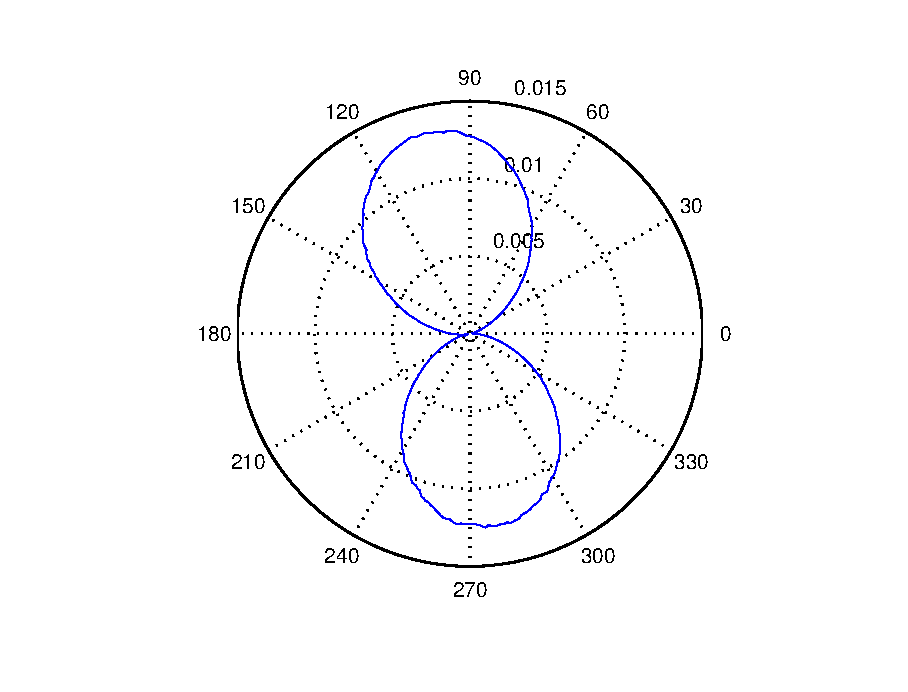
\includegraphics[width=0.7\textwidth]{Plotjes/ass22.eps}
\caption{Polarization pattern of a vertically polarized wave, reflections absorbed}\label{fig:ass22}
\end{figure}

\subsection{Assignment 2.3}\label{ass23}
\begin{figure}[H]
\centering
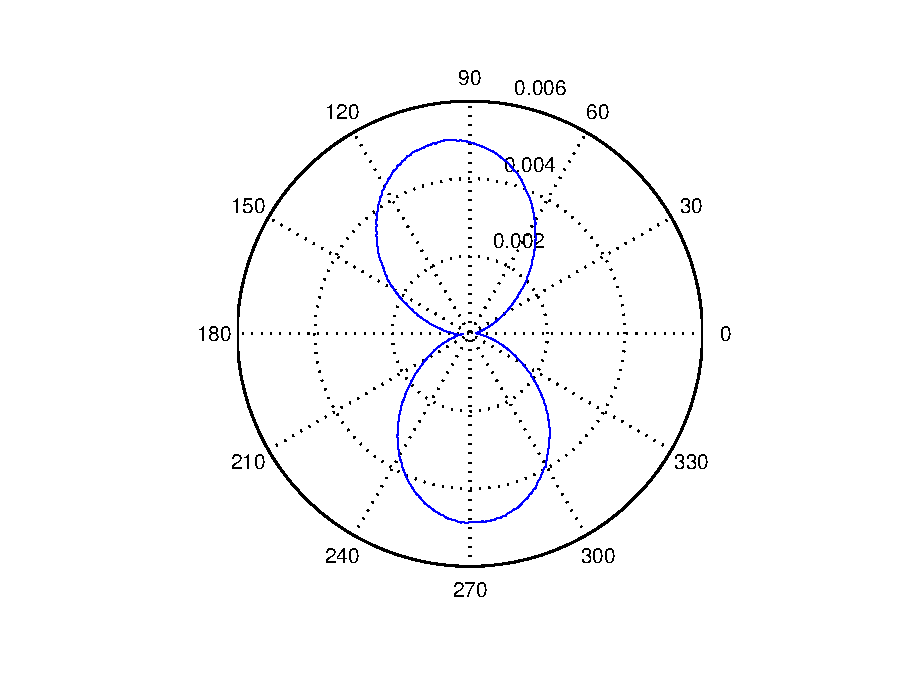
\includegraphics[width=0.8\textwidth]{Plotjes/ass23.eps}
\caption{Polarization pattern of a vertically polarized wave, with metal plate reflector}\label{fig:ass23}
\end{figure}
When comparing \autoref{fig:ass22} and \autoref{fig:ass23}, one can conclude that the metal plate had a significant impact on the amplitude of the signal, but not on the phase. The amplitude in \ref{ass23} is about 2.5 times lower than the original. 

\subsection{Assignment 2.4}
\begin{figure}[H]
\centering
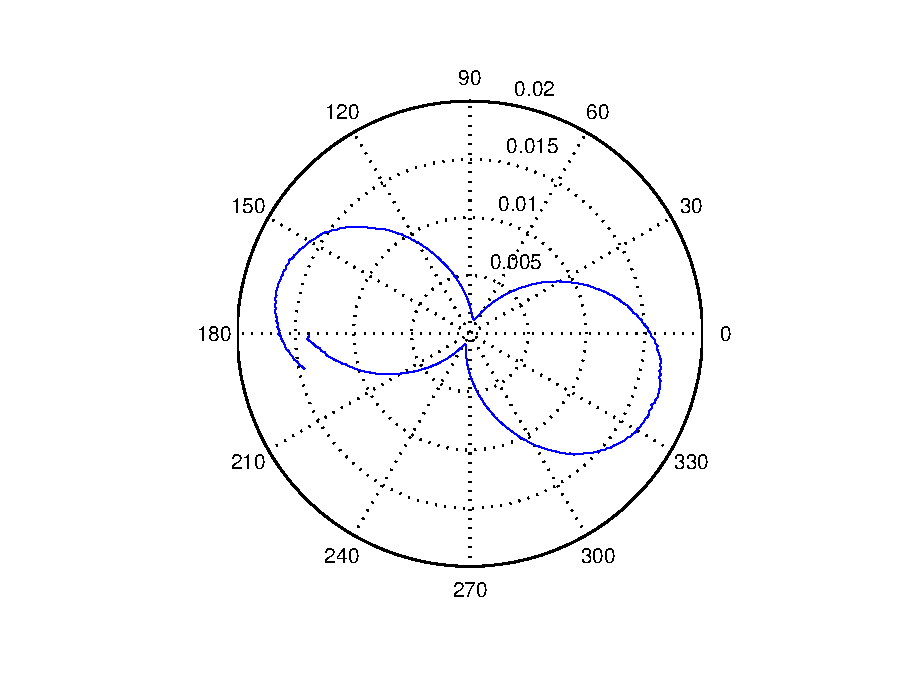
\includegraphics[width=0.7\textwidth]{Plotjes/ass24.eps}
\caption{Polarization pattern of a circular polarized wave, with metal plate reflector. }\label{fig:ass24}
\end{figure}
A circular polarized wave consists of a horizontal and a vertical wave with a phase shift. As seen in \autoref{ass23}, the vertical wave decays significantly due to the metal sheet. When transmitting a circular polarized wave with the same setup as \nameref{ass23}, the resulting wave is mostly horizontally polarized. This can be seen in \autoref{fig:ass24}

\subsection{Assignment 2.5}
\begin{figure}[H]
\centering
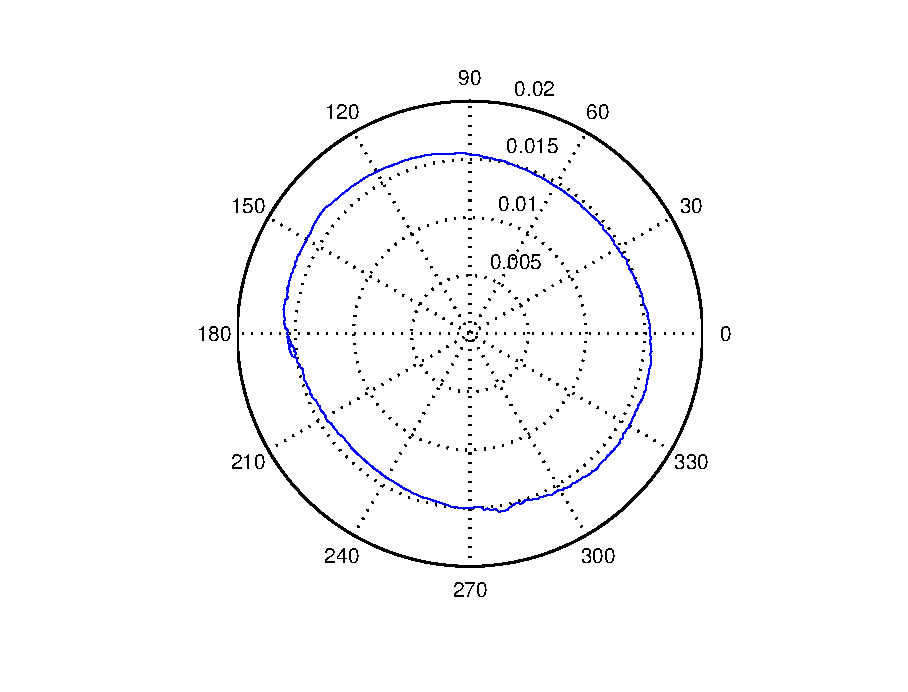
\includegraphics[width=0.7\textwidth]{Plotjes/ass25.eps}
\caption{Polarization pattern of a circular polarized wave, with dielectric plate}
\end{figure}
With the dielectric as reflective sheet, the amplitude of the signal actually increases compared to the case in \nameref{ass21}. 
Also, the polarization is rounder than in \nameref{ass21}. This is because the Axial Ratio is closer to 1. \\
The Axial Ratio can be calculated with $AR = V_{max}/V_{min}$. A table containing these values can be found in Table \ref{tab:AR}. As it approaches infinity, the polarization pattern will look more like an 8. This is seen in Figure \ref{fig:ass24}. As it becomes lower, the polarization pattern will look more circular. 

		\begin{table}[H]
			\centering
			\begin{tabular}{l|llllll}
				                       & Nothing        & Metal         & Dielectric & \\ \hline
				Axial Ratio & 1.32        & 17.2            & 1.18\\
			\end{tabular}
			\caption{Axial Ratios of the reflectors}
			\label{tab:AR}
		\end{table}

\section{Reflection Coefficient Calculation}

The recieved amplitude at \autoref{ass23} was 2.63 times lower than in \autoref{ass22}. Equivalently:
 
 $$ A_{Vmetal} = 0.38\cdot A $$
 \begin{subequations}
and since
\begin{align}
 E_{0r} = A\left| 1+\Gamma e^{-j2kh_1h_2/d}\right|
 \end{align}
We can calculate $\Gamma_{Vmetal}$ from this:
\begin{align}
 A_{Vmetal} &= A \left| 1 + \Gamma_{Vmetal}\cdot e^{-2j\cdot k \cdot h_1 h_2 / d} \right| \\
 0.38 &=   \left| 1 + \Gamma_{Vmetal}\cdot e^{-2j\cdot k \cdot h_1 h_2 / d} \right| 
 \end{align}
 With $h_1 = h_2 = 0.155m$ and $d = 1.86m$ this results in $\Gamma_{Vmetal} = -0.13 + 0.6062i $. 
\end{subequations}
%\appendix
%\section{Measured data}
%Using equation 2.1 from the manual %TODO bibtex
%we can derive the following relations:
%
%$$ E_{0r} = A\left| 1+\Gamma e^{-j2kh_1h_2/d}\right| $$
%with 
%$$ k = \dfrac{2\pi}{\lambda} = \dfrac{2\pi f}{v} $$
%With $f$ the frequency of the wave and $v$ the propagation speed of air.
%%$$ k = \dfrac{2\pi \cdot 9.1\cdot 10^{9}}{3\cdot 10^{8}} = $$
%Furthermore, $h_1$ and $h_2$ are defined as the height difference between the metal sheet and respectively the transmitting antenna and recieving antenna and $d$ the distance between the antennas. These parameters where measured during the assignment and were found to be $h_1 = h_2 = 0.155\si{\meter}$ and $d = 1.86\si{\meter}$

\end{document}
